% Options for packages loaded elsewhere
\PassOptionsToPackage{unicode}{hyperref}
\PassOptionsToPackage{hyphens}{url}
\PassOptionsToPackage{dvipsnames,svgnames,x11names}{xcolor}
%
\documentclass[
  letterpaper,
  DIV=11,
  numbers=noendperiod]{scrartcl}

\usepackage{amsmath,amssymb}
\usepackage{iftex}
\ifPDFTeX
  \usepackage[T1]{fontenc}
  \usepackage[utf8]{inputenc}
  \usepackage{textcomp} % provide euro and other symbols
\else % if luatex or xetex
  \usepackage{unicode-math}
  \defaultfontfeatures{Scale=MatchLowercase}
  \defaultfontfeatures[\rmfamily]{Ligatures=TeX,Scale=1}
\fi
\usepackage{lmodern}
\ifPDFTeX\else  
    % xetex/luatex font selection
  \setmainfont[]{Trixie-Text}
  \setsansfont[]{Trixie-Text}
  \setmonofont[]{Trixie-Text}
\fi
% Use upquote if available, for straight quotes in verbatim environments
\IfFileExists{upquote.sty}{\usepackage{upquote}}{}
\IfFileExists{microtype.sty}{% use microtype if available
  \usepackage[]{microtype}
  \UseMicrotypeSet[protrusion]{basicmath} % disable protrusion for tt fonts
}{}
\makeatletter
\@ifundefined{KOMAClassName}{% if non-KOMA class
  \IfFileExists{parskip.sty}{%
    \usepackage{parskip}
  }{% else
    \setlength{\parindent}{0pt}
    \setlength{\parskip}{6pt plus 2pt minus 1pt}}
}{% if KOMA class
  \KOMAoptions{parskip=half}}
\makeatother
\usepackage{xcolor}
\usepackage[left=.5in,textwidth=5.5in,marginparsep=.25in,marginparwidth=2.25in]{geometry}
\setlength{\emergencystretch}{3em} % prevent overfull lines
\setcounter{secnumdepth}{-\maxdimen} % remove section numbering
% Make \paragraph and \subparagraph free-standing
\ifx\paragraph\undefined\else
  \let\oldparagraph\paragraph
  \renewcommand{\paragraph}[1]{\oldparagraph{#1}\mbox{}}
\fi
\ifx\subparagraph\undefined\else
  \let\oldsubparagraph\subparagraph
  \renewcommand{\subparagraph}[1]{\oldsubparagraph{#1}\mbox{}}
\fi


\providecommand{\tightlist}{%
  \setlength{\itemsep}{0pt}\setlength{\parskip}{0pt}}\usepackage{longtable,booktabs,array}
\usepackage{calc} % for calculating minipage widths
% Correct order of tables after \paragraph or \subparagraph
\usepackage{etoolbox}
\makeatletter
\patchcmd\longtable{\par}{\if@noskipsec\mbox{}\fi\par}{}{}
\makeatother
% Allow footnotes in longtable head/foot
\IfFileExists{footnotehyper.sty}{\usepackage{footnotehyper}}{\usepackage{footnote}}
\makesavenoteenv{longtable}
\usepackage{graphicx}
\makeatletter
\def\maxwidth{\ifdim\Gin@nat@width>\linewidth\linewidth\else\Gin@nat@width\fi}
\def\maxheight{\ifdim\Gin@nat@height>\textheight\textheight\else\Gin@nat@height\fi}
\makeatother
% Scale images if necessary, so that they will not overflow the page
% margins by default, and it is still possible to overwrite the defaults
% using explicit options in \includegraphics[width, height, ...]{}
\setkeys{Gin}{width=\maxwidth,height=\maxheight,keepaspectratio}
% Set default figure placement to htbp
\makeatletter
\def\fps@figure{htbp}
\makeatother

\KOMAoption{captions}{tableheading}
\makeatletter
\makeatother
\makeatletter
\makeatother
\makeatletter
\@ifpackageloaded{caption}{}{\usepackage{caption}}
\AtBeginDocument{%
\ifdefined\contentsname
  \renewcommand*\contentsname{Table of contents}
\else
  \newcommand\contentsname{Table of contents}
\fi
\ifdefined\listfigurename
  \renewcommand*\listfigurename{List of Figures}
\else
  \newcommand\listfigurename{List of Figures}
\fi
\ifdefined\listtablename
  \renewcommand*\listtablename{List of Tables}
\else
  \newcommand\listtablename{List of Tables}
\fi
\ifdefined\figurename
  \renewcommand*\figurename{Figure}
\else
  \newcommand\figurename{Figure}
\fi
\ifdefined\tablename
  \renewcommand*\tablename{Table}
\else
  \newcommand\tablename{Table}
\fi
}
\@ifpackageloaded{float}{}{\usepackage{float}}
\floatstyle{ruled}
\@ifundefined{c@chapter}{\newfloat{codelisting}{h}{lop}}{\newfloat{codelisting}{h}{lop}[chapter]}
\floatname{codelisting}{Listing}
\newcommand*\listoflistings{\listof{codelisting}{List of Listings}}
\makeatother
\makeatletter
\@ifpackageloaded{caption}{}{\usepackage{caption}}
\@ifpackageloaded{subcaption}{}{\usepackage{subcaption}}
\makeatother
\makeatletter
\@ifpackageloaded{tcolorbox}{}{\usepackage[skins,breakable]{tcolorbox}}
\makeatother
\makeatletter
\@ifundefined{shadecolor}{\definecolor{shadecolor}{rgb}{.97, .97, .97}}
\makeatother
\makeatletter
\makeatother
\makeatletter
\makeatother
\ifLuaTeX
  \usepackage{selnolig}  % disable illegal ligatures
\fi
\IfFileExists{bookmark.sty}{\usepackage{bookmark}}{\usepackage{hyperref}}
\IfFileExists{xurl.sty}{\usepackage{xurl}}{} % add URL line breaks if available
\urlstyle{same} % disable monospaced font for URLs
\hypersetup{
  pdftitle={\_\_\_\_\_\_\_\_\_\_\_\_\_\_\_\_\_\_\_\_\_\_\_\_\_\_\_\_\_\_\_\_\_\_\_\_\_\_\_\_\_},
  pdfauthor={Prueba 2 SOL114},
  colorlinks=true,
  linkcolor={blue},
  filecolor={Maroon},
  citecolor={Blue},
  urlcolor={Blue},
  pdfcreator={LaTeX via pandoc}}

\title{\_\_\_\_\_\_\_\_\_\_\_\_\_\_\_\_\_\_\_\_\_\_\_\_\_\_\_\_\_\_\_\_\_\_\_\_\_\_\_\_\_}
\author{Prueba 2 SOL114}
\date{}

\begin{document}
\maketitle
\ifdefined\Shaded\renewenvironment{Shaded}{\begin{tcolorbox}[breakable, interior hidden, borderline west={3pt}{0pt}{shadecolor}, enhanced, frame hidden, boxrule=0pt, sharp corners]}{\end{tcolorbox}}\fi

\begin{enumerate}
\def\labelenumi{\arabic{enumi}.}
\tightlist
\item
  (8\%) Dado un estimador \(\hat{\theta}\), el Error Cuadrático Medio
  (MSE) es una forma de cuantificar la bondad de este estimador.
  Formalmente el MSE se define como:
\end{enumerate}

\[\text{MSE}(\hat{\theta}) = \mathbb{E}[(\hat{\theta} - \theta)^2]\]

Después de un poco de álgebra el MSE puede ser descompuesto en dos
componentes:

\[\text{MSE}(\hat{\theta}) = \underbrace{\mathbb{E}[(\hat{\theta} - \mathbb{E}[\hat{\theta}])^2]}_{\framebox[5cm][l]{Varianza}} + \overbrace{(\mathbb{E}[\hat{\theta} - \theta ])^2}^{\framebox[5cm][l]{Sesgo al cuadrado}}\]

\begin{enumerate}
\def\labelenumi{\roman{enumi}.}
\item
  Explica en palabras lo que mide el MSE: El MSE mide, en términos
  generales, cuánto se espera que las estimaciones de \(\hat{\theta}\)
  difieran del valor verdadero \(\theta\) al cuadrado. En otras
  palabras, cuantifica la cantidad promedio de error cuadrático en las
  estimaciones de \(\hat{\theta}\) en relación con el valor verdadero
  \(\theta\). Un MSE más bajo indica que las estimaciones son más
  precisas y se acercan más al valor verdadero, mientras que un MSE más
  alto indica estimaciones menos precisas y más alejadas del valor
  verdadero.
\item
  Identifica y explica en qué consiste cada uno de sus componentes:
\end{enumerate}

El primer componente,
\(\mathbb{E}[(\hat{\theta} - \mathbb{E}[\hat{\theta}])^2]\), representa
la varianza de las estimaciones de \(\hat{\theta}\). Esta parte del MSE
mide cuánto las estimaciones individuales fluctúan alrededor de su valor
promedio, es decir, cuánta dispersión hay en las estimaciones. Cuanto
mayor sea esta varianza, mayor será la dispersión de las estimaciones
alrededor de su valor promedio, lo que indica una menor precisión.

El segundo componente, \((\mathbb{E}[\hat{\theta} - \theta])^2\), es el
sesgo al cuadrado de las estimaciones. El sesgo se refiere a la
diferencia sistemática entre el valor esperado de las estimaciones y el
valor verdadero (\(\theta\)). Elevar al cuadrado el sesgo y tomar su
esperanza cuantifica cuánto se aleja, en promedio, la estimación del
valor verdadero al cuadrado. Un sesgo cuadrado más alto indica que las
estimaciones tienden a estar sistemáticamente más lejos del valor
verdadero.

En resumen, el MSE mide la calidad de un estimador al descomponerla en
dos componentes: la varianza de las estimaciones (cuánto fluctúan
alrededor de su promedio) y el sesgo al cuadrado (cuánto se alejan en
promedio del valor verdadero). Un buen estimador tendrá un MSE bajo, lo
que significa que tiene una baja varianza y un sesgo cercano a cero, lo
que indica estimaciones precisas y no sesgadas.

\begin{enumerate}
\def\labelenumi{\arabic{enumi}.}
\setcounter{enumi}{1}
\tightlist
\item
  (12\%) A pesar de que el peso de una vaca individual depende de
  factores idiosincráticos, diferentes razas de vacas presentan
  distintos pesos promedios (debido factores ambientales y genéticos).
  En particular, los zoólogos han determinado que el peso de las
  terneras de la raza Milking Shorthorn (a los 2 años de vida) puede ser
  descrito con una distribución normal con media \(\mu=500\) kg y
  desviación estándar \(\sigma=65\) kg.
\end{enumerate}

\begin{figure}

{\centering 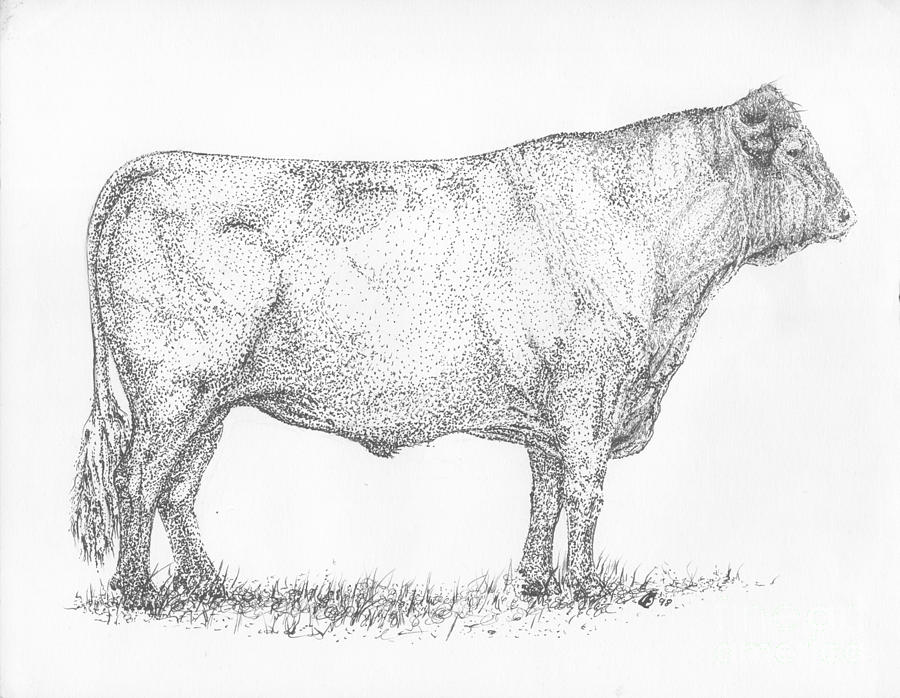
\includegraphics[width=10cm,height=\textheight]{vaca.jpg}

}

\caption{Milking Shorthorn}

\end{figure}

Un ganadero de Yorkshire tiene 196 terneras de la raza Milking Shorthorn
y decide calcular el peso promedio de sus vacas (\(\bar{X}\)). Como
resultado obteniene \(\bar{X}=491\).

\begin{enumerate}
\def\labelenumi{\roman{enumi}.}
\tightlist
\item
  Deriva la distribución muestral de \(\bar{X}\): La distribución
  muestral de \(\bar{X}\), el promedio de las muestras de tamaño \(n\)
  tomadas de una población con una distribución normal con media \(\mu\)
  y desviación estándar \(\sigma\), sigue una distribución normal con
  media \(\mu_{\bar{X}} = \mu\) (la misma que la población) y desviación
  estándar \(\sigma_{\bar{X}} = \frac{\sigma}{\sqrt{n}}\). En este caso,
  \(\mu = 500\) kg, \(\sigma = 65\) kg, y \(n = 196\) terneras, por lo
  que:
\end{enumerate}

\[\mu_{\bar{X}} = 500 \text{ kg}\]
\[\sigma_{\bar{X}} = \frac{65}{\sqrt{196}} = \frac{65}{14} \text{ kg} = 4.642 \text{ kg}\]

\begin{enumerate}
\def\labelenumi{\roman{enumi}.}
\setcounter{enumi}{1}
\tightlist
\item
  Calcula un intervalo de confianza al 99\% para el promedio estimado
  por el ganadero de Yorkshire: Para calcular un intervalo de confianza
  al 99\% para el promedio estimado por el ganadero (\(\bar{X}\)),
  podemos usar la fórmula del intervalo de confianza para la media:
\end{enumerate}

\[\bar{X} \pm Z \frac{\sigma}{\sqrt{n}}\]

Donde: - \(\bar{X}\) es el promedio muestral observado, que es \(491\)
kg. - \(Z\) es el valor crítico correspondiente al nivel de confianza
del 99\%. Podemos encontrar este valor usando una tabla de distribución
normal estándar. Para un nivel de confianza del 99\%,
\(Z \approx 2.576\). - \(\sigma\) es la desviación estándar de la
población, que es \(65\) kg. - \(n\) es el tamaño de la muestra, que es
\(196\) terneras.

Sustituyendo los valores:

\[\bar{X} \pm 2.576 \frac{65}{\sqrt{196}} = 491 \pm 2.576 \frac{65}{14} \text{ kg}\]

Calculando los límites del intervalo:

Límite inferior: \(491 - 2.576 \frac{65}{14} \approx 491\) kg Límite
superior: \(491 + 2.576 \frac{65}{14} \approx 503\) kg

Por lo tanto, el intervalo de confianza al 99\% para el promedio de peso
estimado por el ganadero es aproximadamente
\((491 \text{ kg}, 503 \text{ kg})\).

\begin{enumerate}
\def\labelenumi{\roman{enumi}.}
\setcounter{enumi}{2}
\tightlist
\item
  En base a los resultados, ¿podemos decir que las terneras del ganadero
  tienen un peso estadísticamente inferior, similar o superior al peso
  esperado para las terneras de esta raza?:
\end{enumerate}

Dado que el intervalo de confianza al 99\% incluye el valor esperado
para las terneras de la raza Milking Shorthorn (\(\mu = 500\) kg), no
podemos afirmar que las terneras del ganadero tengan un peso
estadísticamente inferior. El intervalo de confianza incluye el valor
esperado, lo que sugiere que el peso promedio estimado por el ganadero
es estadísticamente similar al peso esperado para las terneras de esta
raza.

\begin{enumerate}
\def\labelenumi{\arabic{enumi}.}
\setcounter{enumi}{2}
\tightlist
\item
  (8\%) Siguiendo con la pregunta anterior, ¿Cual es la probabilidad de
  que el peso promedio obtenido por el ganadero con una muestra de 196
  terneras sea menor que la media poblacional (\(\mu\)) en al menos
  10kg?
\end{enumerate}

Para encontrar la probabilidad de que el peso promedio obtenido por el
ganadero con una muestra de 196 terneras sea menor que la media
poblacional (\(\mu\)) en al menos 10 kg, primero necesitamos calcular la
probabilidad de que la media muestral sea menor que \(\mu - 10\) kg.

Dado que la distribución muestral de \(\bar{X}\) es normal con media
\(\mu_{\bar{X}} = \mu\) y desviación estándar
\(\sigma_{\bar{X}} = \frac{\sigma}{\sqrt{n}}\), podemos estandarizar el
valor \(\mu - 10\) kg utilizando la fórmula Z:

\[Z = \frac{\bar{X} - \mu}{\sigma_{\bar{X}}}\]

En este caso:

\[Z = \frac{(\mu - 10) - \mu}{\frac{\sigma}{\sqrt{n}}} = \frac{-10}{\frac{65}{\sqrt{196}}} = \frac{-10}{\frac{65}{14}} = -\frac{140}{65} \approx -2.154\]

Ahora, queremos encontrar la probabilidad de que \(Z\) sea menor que
\(-2.154\), lo que equivale a encontrar el área bajo la curva de la
distribución normal estándar a la izquierda de \(Z = -2.154\).

La probabilidad de que \(Z\) sea menor que \(-2.154\) es aproximadamente
0.016. Esto significa que la probabilidad de que el peso promedio
obtenido por el ganadero con una muestra de 196 terneras sea menor que
la media poblacional en al menos 10 kg es aproximadamente 1.6\%.

\begin{enumerate}
\def\labelenumi{\arabic{enumi}.}
\setcounter{enumi}{3}
\tightlist
\item
  (15\%) La siguiente tabla reporta los resultados de una muestra
  aleatoria de 10 estudiantes en el curso SOL3212.
\end{enumerate}

\begin{longtable}[]{@{}llll@{}}
\toprule\noalign{}
Estudiante & Prueba 1 & Prueba 2 & Nota final \\
\midrule\noalign{}
\endhead
\bottomrule\noalign{}
\endlastfoot
Juan & 6.5 & 6.2 & 6.35 \\
María & 5.8 & 5.5 & 5.65 \\
Carlos & 6.7 & 5.9 & 6.3 \\
Ana & 6.0 & 5.4 & 5.7 \\
Felipe & 4.5 & 5.0 & 4.75 \\
Sofia & 6.8 & 6.7 & 6.75 \\
Gabriel & 5.2 & 5.9 & 5.55 \\
Valeria & 6.3 & 6.5 & 6.4 \\
Roberto & 5.0 & 5.3 & 5.15 \\
Laura & 6.4 & 6.6 & 6.5 \\
\(\sum{x_i}\) & \textbf{59.4} & \textbf{58.9} & \textbf{59.15} \\
\(\sum{(x_i - \overline{x})^2}\) & \textbf{2.475} & \textbf{2.41} &
\textbf{0.5475} \\
\end{longtable}

\begin{enumerate}
\def\labelenumi{\roman{enumi}.}
\tightlist
\item
  Calcula un intervalo al 97\% de confianza para las Pruebas 1 y 2: Para
  calcular los intervalos de confianza al 97\% para las Pruebas 1 y 2,
  utilizaremos la fórmula del intervalo de confianza para la media
  poblacional cuando la muestra es pequeña y/o la varianza poblacional
  es desconocida. La fórmula es la siguiente:
\end{enumerate}

\[\text{Intervalo de Confianza} = \overline{x} \pm t_{\frac{\alpha}{2}, n-1} \left(\frac{s}{\sqrt{n}}\right)\]

Donde: - \(\overline{x}\) es la media de la muestra. -
\(t_{\frac{\alpha}{2}, n-1}\) es el valor crítico de la distribución t
de Student con \(n-1\) grados de libertad y \(\alpha/2\) de probabilidad
en la cola izquierda. Para un nivel de confianza del 97\%,
\(\alpha = 0.03\) y \(n\) es el tamaño de la muestra. - \(s\) es la
desviación estándar de la muestra. - \(n\) es el tamaño de la muestra.

Para Prueba 1: - \(\overline{x}_1 = 5.94\) (promedio de Prueba 1) -
\(s_1 = \sqrt{\frac{\sum{(x_i - \overline{x}_1)^2}}{n-1}} = \sqrt{\frac{2.475}{10-1}} \approx 0.524\)
(desviación estándar de Prueba 1) - \(n_1 = 10\) (tamaño de la muestra)

Para Prueba 2: - \(\overline{x}_2 = 5.89\) (promedio de Prueba 2) -
\(s_2 = \sqrt{\frac{\sum{(x_i - \overline{x}_2)^2}}{n-1}} = \sqrt{\frac{2.41}{10-1}} \approx 0.517\)
(desviación estándar de Prueba 2) - \(n_2 = 10\) (tamaño de la muestra)

Para un nivel de confianza del 97\%, el valor crítico de
\(t_{\frac{\alpha}{2}, n-1}\) es aproximadamente \(2.57\) para
\(n-1 = 9\) grados de libertad.

Calculamos los intervalos de confianza:

Para Prueba 1:
\[\text{Intervalo de Confianza para Prueba 1} = 5.94 \pm 2.57 \left(\frac{0.524}{\sqrt{10}}\right) \approx (5.42, 6.37)\]

Para Prueba 2:
\[\text{Intervalo de Confianza para Prueba 2} = 5.89 \pm 2.57 \left(\frac{0.517}{\sqrt{10}}\right) \approx (5.47, 6.31)\]

\begin{enumerate}
\def\labelenumi{\roman{enumi}.}
\setcounter{enumi}{1}
\tightlist
\item
  Compara los intervalos para ambas pruebas y elabora una conclusión
  sustantiva (corta) en base a dicha comparación:
\end{enumerate}

\begin{itemize}
\tightlist
\item
  Los intervalos de confianza para ambas pruebas se superponen
  significativamente, lo que significa que no hay una diferencia
  estadísticamente significativa entre las medias de las dos pruebas.
\item
  Esto sugiere que, con un nivel de confianza del 97\%, no podemos
  concluir que una de las pruebas sea significativamente diferente de la
  otra en términos de la puntuación promedio.
\end{itemize}

\begin{enumerate}
\def\labelenumi{\arabic{enumi}.}
\setcounter{enumi}{4}
\tightlist
\item
  (15\%) El instituto de sociología encarga un estudio de mayor escala
  sobre el rendimiento de los estudiantes en el curso SOL3212. Para
  dicho estudio un psicólogo toma una muestra aleatoria de 484
  estudiantes y calcula los siguientes estadísticos en bases a su
  muestra:
\end{enumerate}

\begin{itemize}
\item
  Nota final, denotada como
  \(X = (\text{Prueba 1} + \text{Prueba 2})/2\):
\item
  Promedio de la muestra de notas finales: \(\bar{X} = 5.9\)
\item
  Desviación estándar de la muestra de notas finales:
  \(\hat{\sigma}_{\text{naive}} = 0.5\)

  \begin{enumerate}
  \def\labelenumi{\roman{enumi}.}
  \item
    Dado que el psicólogo no pasó por el curso SOL114, es posible que
    sus estimaciones no sean del todo correctas. En particular, indica
    si la desviación estándar provista por el psicólogo es o no un
    estimador insesgado de la desviación estándar poblacional
    (\(\sigma\)) y fundamenta tu respuesta.
  \item
    Calcula un intervalo de confianza al 95\% para el promedio muestral
    \(\bar{X} = 5.9\). Explica qué signica dicho intervalo en términos
    estadísticos.
  \end{enumerate}
\end{itemize}

\begin{enumerate}
\def\labelenumi{\roman{enumi}.}
\tightlist
\item
  La desviación estándar muestral proporcionada por el psicólogo
  (\(\hat{\sigma}_{\text{naive}} = 0.5\)) no es un estimador insesgado
  de la desviación estándar poblacional (\(\sigma\)). La razón de esto
  es que la fórmula utilizada para calcular
  \(\hat{\sigma}_{\text{naive}}\) no ajusta el divisor por la pérdida de
  un grado de libertad.
\end{enumerate}

La desviación estándar poblacional (\(\sigma\)) se estima mediante la
fórmula de desviación estándar insesgada corregida:

\[\hat{\sigma} = \sqrt{\frac{n}{n-1}\left(\frac{\sum{(x_i - \bar{x})^2}}{n}\right)} = \sqrt{\frac{484}{484-1}0.5^2} = 0.5005173\]

En esta fórmula, el factor de corrección n/(n-1) se utiliza para ajustar
la desviación estándar muestral y hacerla insesgada.

\begin{enumerate}
\def\labelenumi{\roman{enumi}.}
\setcounter{enumi}{1}
\tightlist
\item
  Ahora, calculamos el intervalo de confianza al 95\% para el promedio
  muestral \(\bar{X} = 5.9\) utilizando la fórmula corregida:
\end{enumerate}

\[\text{Intervalo de Confianza} = \bar{X} \pm t_{\frac{\alpha}{2}, n-1} \frac{\hat{\sigma}}{\sqrt{n}}\]

Donde: - \(\bar{X}\) es la media muestral observada, que es \(5.9\). -
\(t_{\frac{\alpha}{2}, n-1}\) es el valor crítico de la distribución t
de Student con \(n-1\) grados de libertad y \(\alpha/2\) de probabilidad
en la cola izquierda. Para un nivel de confianza del 95\%,
\(\alpha = 0.05\) y \(n\) es el tamaño de la muestra, que es \(484\)
estudiantes. - \(\hat{\sigma}\) es la desviación estándar muestral
estimada con corrección n/(n-1).

Luego, calculamos el valor crítico de t para un nivel de confianza del
95\% con 483 grados de libertad. Puedes encontrar este valor utilizando
una tabla de distribución t-student. Para el nivel de confianza del
95\%, \(t_{\frac{\alpha}{2}, 483} \approx 1.964\).

Sustituyendo los valores en la fórmula del intervalo de confianza:

\[\text{Intervalo de Confianza} = 5.9 \pm 1.964 \frac{0.501}{\sqrt{484}}\]

Calculando los límites del intervalo:

Límite inferior: \(\approx 5.86\), Límite superior: \(\approx 5.95\).

En términos estadísticos, este intervalo significa que con un nivel de
confianza del 95\%, podemos afirmar que el promedio de notas finales de
la población de estudiantes en el curso SOL3212 se encuentra dentro del
rango de 5.86 a 5.95, basado en la muestra de 484 estudiantes.

\begin{enumerate}
\def\labelenumi{\arabic{enumi}.}
\setcounter{enumi}{5}
\tightlist
\item
  (15\%) La consultora CALLEMP lleva a cabo una encuesta en dos comunas,
  VyT y ÑuÑ, para medir la intención de voto en un plebiscito con dos
  opciones: ``A favor'' y ``En contra''. En la comuna VyT los resultados
  de la encuesta sugieren que la opción ``A favor'' ganará claramente,
  mientras que en la comuna ÑuÑ, la opción ``En contra'' obtendría una
  clara ventaja. A continuación, se presenta una tabla con los
  resultados de la encuenta para ambas comunas:
\end{enumerate}

\begin{longtable}[]{@{}lll@{}}
\toprule\noalign{}
Comuna & Opción ``A favor'' & Opción ``En contra'' \\
\midrule\noalign{}
\endhead
\bottomrule\noalign{}
\endlastfoot
Vyt & 80 & 20 \\
ÑuÑ & 30 & 70 \\
\end{longtable}

\begin{figure}

{\centering 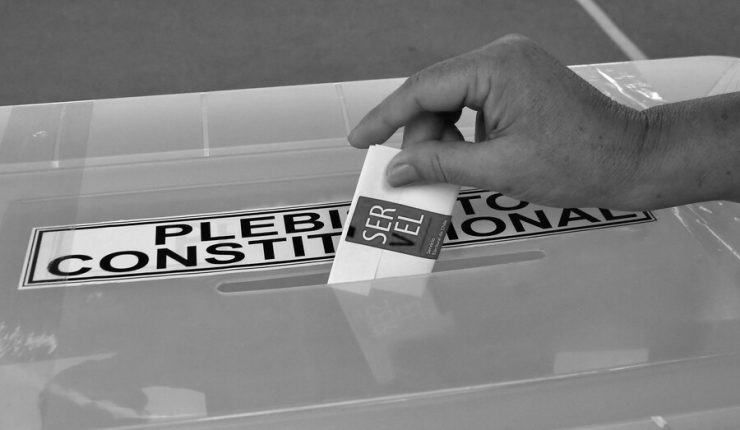
\includegraphics[width=10cm,height=\textheight]{const.png}

}

\caption{Plebiscito}

\end{figure}

\begin{enumerate}
\def\labelenumi{\roman{enumi}.}
\tightlist
\item
  Calcula la proporción estimada de individuos que declaran que votarán
  ``A favor'' en cada comuna: Para calcular la proporción estimada de
  individuos que declaran que votarán ``A favor'' en cada comuna,
  podemos usar la fórmula de proporción muestral:
\end{enumerate}

\[\hat{p} = \frac{\text{Número de votantes "A favor"}}{\text{Total de votantes}}\]

Para la comuna VyT:
\[\hat{p}_{\text{V}} = \frac{80}{80 + 20} = \frac{80}{100} = 0.8\]

Para la comuna ÑuÑ:
\[\hat{p}_{\text{Ñ}} = \frac{30}{30 + 70} = \frac{30}{100} = 0.3\]

\begin{enumerate}
\def\labelenumi{\roman{enumi}.}
\setcounter{enumi}{1}
\tightlist
\item
  Para cada proporción construye un intervalo de confianza al 90\%: Para
  construir un intervalo de confianza al 90\% para cada proporción,
  utilizamos la fórmula del intervalo de confianza para proporciones
  muestrales. La fórmula general para un intervalo de confianza al nivel
  \((1-\alpha)\) para la proporción poblacional \(p\) es:
\end{enumerate}

\[\hat{p} \pm Z_{\frac{\alpha}{2}} \sqrt{\frac{\hat{p}(1-\hat{p})}{n}}\]

Donde: - \(\hat{p}\) es la proporción muestral estimada. -
\(Z_{\frac{\alpha}{2}}\) es el valor crítico correspondiente al nivel de
confianza \((1-\alpha)\). - \(n\) es el tamaño de la muestra.

Para VyT, con \(\hat{p}_{\text{V}} = 0.8\) y \(n = 100\) (80 + 20), y
para un nivel de confianza del 90\%, el valor crítico
\(Z_{\frac{\alpha}{2}}\) es aproximadamente \(1.645\) (puedes
encontrarlo en una tabla de la distribución normal estándar).

El intervalo de confianza para VyT es:

\[\hat{p}_{\text{V}} \pm 1.645 \sqrt{\frac{0.8(1-0.8)}{100}} \approx 0.8 \pm 0.0658 \approx (0.7342, 0.8658)\]

Para ÑuÑ, con \(\hat{p}_{\text{Ñ}} = 0.3\) y \(n = 100\) (30 + 70), y
para un nivel de confianza del 90\%, el valor crítico
\(Z_{\frac{\alpha}{2}}\) es aproximadamente \(1.645\).

El intervalo de confianza para ÑuÑ es:

\[\hat{p}_{\text{Ñ}} \pm 1.645 \sqrt{\frac{0.3(1-0.3)}{100}} \approx 0.3 \pm 0.0754 \approx (0.2246, 0.3753)\]

\begin{enumerate}
\def\labelenumi{\roman{enumi}.}
\setcounter{enumi}{2}
\tightlist
\item
  Compara ambos intervalos y elabora una conclusión sustantiva en base a
  los resultados:
\end{enumerate}

\begin{itemize}
\tightlist
\item
  El intervalo de confianza para VyT va desde aproximadamente 0.7342 a
  0.8658.
\item
  El intervalo de confianza para ÑuÑ va desde aproximadamente 0.2246 a
  0.3753.
\end{itemize}

Con un nivel de confianza del 90\%, podemos estar seguros de que en una
comuna (VyT) ganará la opción ``A favor'', y en la otra comuna (ÑuÑ)
ganará la opción ``En contra''. Los intervalos de confianza respaldan la
predicción de resultados basados en las estimaciones muestrales y la
certeza que ofrecen en términos de las preferencias de voto en ambas
comunas.

\begin{enumerate}
\def\labelenumi{\arabic{enumi}.}
\setcounter{enumi}{6}
\tightlist
\item
  (12\%) La consultora CALLEMP decide elevar el nivel de rigurosidad de
  sus estimaciones. Para ello contratan una socióloga UC a cargo de
  rediseñar el estudio sobre intención de voto. En particular, se le
  pide a la socióloga que, trabajando al 99\% de confianza, reduzca el
  margen de error a 1 punto porcentual.
\end{enumerate}

\begin{enumerate}
\def\labelenumi{\roman{enumi}.}
\item
  Explica el concepto de márgen de error: El margen de error es una
  medida de la incertidumbre asociada a una estimación basada en una
  muestra de datos. Representa cuánto puede variar la estimación
  muestral con respecto al valor real o poblacional. En otras palabras,
  el margen de error corresponde a la mitad de la amplitud de un
  intervalo de confianza. Cuanto menor sea el margen de error, mayor
  será la precisión de la estimación.
\item
  Calcula el tamaño muestral necesario para satisfacer la demanda
  presentada por la consultora y justifica tus decisiones metodológicas:
  Para calcular el tamaño muestral necesario para satisfacer la demanda
  de un margen de error de 1 punto porcentual al 99\% de confianza,
  podemos utilizar la fórmula para el tamaño de muestra en estudios de
  proporciones:
\end{enumerate}

\[n = \frac{Z^2 \cdot p \cdot (1-p)}{E^2}\]

Donde: - \(n\) es el tamaño de la muestra necesario. - \(Z\) es el valor
crítico de la distribución normal estándar correspondiente al nivel de
confianza del 99\%. Para un nivel de confianza del 99\%,
\(Z \approx 2.576\). - \(p(1-p)\) es la varianza de la variable de
interés en la población. Dado que no conocemos esta cantidad usamos una
estimación conservadora de la varianza: varianza máxima (cuando
\(p=0.5\)). - \(E\) es el margen de error deseado, que en este caso es 1
punto porcentual, por lo que \(E = 0.01\).

Sustituyendo los valores en la fórmula:

\[n = \frac{2.576^2 \cdot 0.5 \cdot (1-0.5)}{0.01^2} \approx \frac{1.658724}{0.0001} \approx 16587\]

Dado que el tamaño de la muestra debe ser un número entero, redondeamos
hacia arriba a \(n = 16587\). Por lo tanto, se necesitaría una muestra
de al menos 16,587 observaciones para satisfacer la demanda de un margen
de error de 1 punto porcentual al 99\% de confianza. Esta decisión se
basa en la fórmula estándar de cálculo del tamaño muestral en estudios
de proporciones, asumiendo una proporción conservadora de 0.5 y un nivel
de confianza del 99\%. El objetivo es garantizar que la estimación sea
altamente precisa y confiable.

\begin{enumerate}
\def\labelenumi{\arabic{enumi}.}
\setcounter{enumi}{7}
\tightlist
\item
  (15\%) Verdadero o Falso. Si marcas Falso justifica tu respuesta.
\end{enumerate}

\begin{enumerate}
\def\labelenumi{\roman{enumi}.}
\tightlist
\item
  Un intervalo de confianza al 99\% para la media poblacional significa
  que la probabilidad de que la media tome un valor fuera del intervalo
  es de 1\%.
\end{enumerate}

\begin{itemize}
\tightlist
\item[$\square$]
  Verdadero
\item[$\boxtimes$]
  Falso
\end{itemize}

Un intervalo de confianza al 99\% para la media poblacional no significa
que la probabilidad de que la media esté fuera del intervalo sea del
1\%. La media poblacional no es aleatoria, pero la media muestral si,
porque se estima en base a una muestra aleatoria. En realidad, la
interpretación correcta es que si se repitiera el proceso de muestreo y
construcción del intervalo en muchas ocasiones, el 99\% de esos
intervalos contendrían la verdadera media poblacional. Los intervalos de
confianza se basan en la noción de repetición de muestreos y no
proporcionan una probabilidad sobre la ubicación de la media en un solo
intervalo.

\begin{enumerate}
\def\labelenumi{\roman{enumi}.}
\setcounter{enumi}{1}
\tightlist
\item
  El error estándar de un estimador mide la desviación promedio de las
  estimaciones respecto del verdadero parámetro poblacional, incluso si
  el estimador está sesgado.
\end{enumerate}

\begin{itemize}
\tightlist
\item[$\square$]
  Verdadero
\item[$\boxtimes$]
  Falso
\end{itemize}

El error estándar de un estimador mide la variabilidad o dispersión de
las estimaciones que obtendríamos al aplicar ese estimador a múltiples
muestras aleatorias de la misma población. No necesariamente mide la
desviación promedio de las estimaciones con respecto al verdadero
parámetro poblacional. Si el estimador está sesgado, el error estándar
proporciona una medida de cuánto se espera que varíen las estimaciones
alrededor del promedio del valor estimado, el cual no coincide con valor
real del parámetro poblacional.

\begin{enumerate}
\def\labelenumi{\roman{enumi}.}
\setcounter{enumi}{2}
\tightlist
\item
  Un estimador es insesgado si cada vez que lo aplicamos a una muestra
  aleatoria de una misma población entrega un estimado igual al
  verdadero parámetro poblacional.
\end{enumerate}

\begin{itemize}
\tightlist
\item[$\square$]
  Verdadero
\item[$\boxtimes$]
  Falso
\end{itemize}

Un estimador se considera insesgado si, en promedio, produce
estimaciones equivalentes al valor real del parámetro poblacional cuando
se aplica repetidamente a muestras aleatorias de la misma población. Sin
embargo, un estimador insesgado no garantiza que cada estimación
individual sea igual al valor real del parámetro poblacional en cada
muestra. Puede haber variabilidad en las estimaciones individuales, pero
en promedio, se espera que el estimador no tenga sesgo.



\end{document}
